% ------------------------------------------------------------------ appendices
\appendix

\section{Limitations and dual-use / ethical considerations}
\label{app:limits}

\head{What the results establish.} In a simplified sandbox with one model family (gpt-oss-120b) and 10 agents per run, monitors calibrated on independent agents flag fleets that never communicate, and a test calibrated on replicate runs of the same deployment does not, while still recovering logged transmission. Tier B extends the monitors' behaviour to 1,200 agents by resampling real Tier A trajectories; it does not simulate new agent behaviour at that scale.

\head{What they do not establish.}
\begin{itemize}
\item \emph{Replicate runs are an assumption, not a given.} M4 needs several runs of the same deployment whose common causes recur. Evaluation fleets (ExploitGym-style batches) have them; a single long-running production deployment may not, and \texttt{fleet\_drift} shows the test then fails. Within one run, splitting by time window or cohort is the natural substitute, untested here.
\item \emph{Partly circular ground truth.} Transmission is labelled by a copied private endpoint, which is also M4's strongest signal; an exploratory rarity rule using the same replicate-run reference matches M4 (Section~\ref{sec:h2}). The benchmark shows that the reference population removes the fleet trap, not that M4's statistic beats simpler rules.
\item \emph{Shared provenance, not direct edges.} M4 detects that two agents carry information from the same source; siblings who copied one leader are flagged too. Attributing the direct edge needs read logs.
\item \emph{Simplified world.} One task type, one shock, 20 ticks, a board as the only channel, and transmission that leaves an endpoint trace in the API log. Channels that leave no action trace (or encode content steganographically) are outside the test; covert channels are a separate defence.
\item \emph{One cheap model; instructed swarm.} Swarm agents were told to share; emergent sharing was rare (Section~\ref{sec:passing}). The LLM judge is one prompt and one model.
\item \emph{Real data is only a bound.} H4 calibrates an estimator; it cannot show whether the wiki agents communicated (Shalizi and Thomas [6]).
\end{itemize}

\head{Dual use.} A timing- and provenance-based detector tells a coordinating swarm what to hide: jitter its timing, diversify endpoints, or vary its common causes across runs. We publish the benchmark, the test and its failure modes, not evasion strategies; the failure modes are the ones defenders need to know, and they are already implicit in prior work on coordinated-behaviour detection [14]. The sandbox runs only harmless lookups against a fake local API, no agent had internet access, and no third-party personal data was used (we did not download the collusion.wiki operator's request log, which holds third parties' IP addresses). The Swarm Traces attack payloads were not used.

\section{Changes before and after the freeze, and plan items not done}
\label{app:dev}
All changes were made on pilot and dev data, before the main runs, and are logged with reasons in \texttt{plan/deviations.md}: P1--P3 (pilots v1--v3: an outage window instead of a permanent outage, only two ``discoverers'', a one-call board read); P4 (per-condition \texttt{/help} policy, \texttt{wave} and \texttt{tacit}); P5 (deployment-level common causes constant across runs); P6 (from synthetic calibration tests: inverse-frequency token weights, randomized p-values, shuffle surrogates for M3); P7 (from dev data: M3 calibrated on independent agents, G4 made one-sided, the \texttt{fleet\_drift} condition, the M1 judge kept as written although it never flagged on dev). Author decision before the freeze: the swarm gate G1 is episode-level (at least 70\% of swarm episodes contain a verified adoption) and pairs are labelled by observed transmission. \textbf{After the freeze} no frozen file changed (hashes verified). One analysis deviation: the plan calibrated H4 on sandbox wave episodes and Tier B fleets, but 20-tick episodes are too short for a Hawkes fit, so H4 sweeps baseline block widths and calibrates on simulated start-wave and contagion processes matched to the wiki's size (D1 in \texttt{plan/deviations.md}).

\head{Further departures from the plan} (logged in \texttt{plan/deviations.md} as P8 and D4--D6).
\begin{itemize}
\item \emph{Tier B is a resampler, not a fitted simulator (D4).} The plan specified an event simulator whose base rate, shock response and lag distribution were fitted to Tier A. Tier B instead resamples real Tier A agent trajectories (so marginals match exactly) and plants adoption with a fixed 1--3 tick lag; it represents agents by disruption tokens only (503, help, workaround), and estimates rates on 2,000 sampled pairs per setting rather than the planned 20,000. It therefore extrapolates Tier A behaviour; it does not simulate new behaviour.
\item \emph{No minimum detectable coupling (D5).} The plan asked for the smallest detectable $c$. M4's recall is already \nTBFNonetwozerozerocfiveMfourTpr\% at the smallest planted coupling ($c = 0.05$) at every $N$, because planted copies repeat every leader use, while M2 and M3 never reach 80\% at any $c$ (Figure~\ref{fig:scale}b). The quantity is not identified on this grid; we did not extend it.
\item \emph{Rare-endpoint rule (D6).} Added after the freeze at a reviewer's request and labelled exploratory (\texttt{src/analysis/rare\_endpoint\_baseline.py}; Section~\ref{sec:h2}).
\item \emph{Paraphrase dropped (P8).} Paraphrasing transcripts to test M0 and M1 was a stretch item; it was dropped before the freeze, but the decision was logged only afterwards.
\item \emph{Not done.} The planned estimator-audit table, including a sandbox analogue of Lütje's read-before-adopt gap, was not built; its other rows appear separately (Table~\ref{tab:h2}, Section~\ref{sec:h4}). We discuss three public incidents but did not build a case-by-case incident ledger with control cases.
\end{itemize}

\section{Mechanism check: lag profiles}
\label{app:lag}
\begin{figure}[h]
\centering
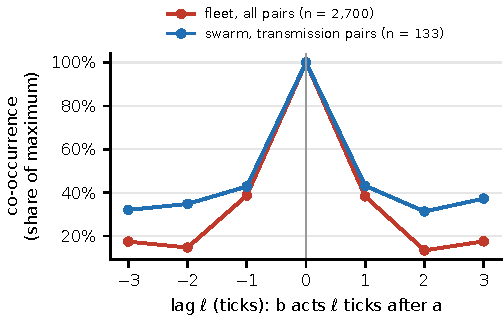
\includegraphics[width=0.5\textwidth]{fig5_lag.pdf}
\vspace{-8pt}
\caption{\label{fig:lag}Raw lagged co-occurrence of disruption tokens (agent $b$ acting $\ell$ ticks after agent $a$), normalised to its maximum, for all fleet pairs and for swarm pairs with logged transmission. Both peak at lag 0: the shared outage, not the transmission, dominates timing. We had predicted a positive-lag peak for transmission pairs; the data does not show one, and the separation in Section~\ref{sec:h2} comes from which endpoints pairs share.}
\end{figure}

\section*{LLM usage statement}
Claude (Anthropic) was used as a research and engineering assistant throughout: literature search and reading, design discussion, writing and testing the code, running the experiments, analysis, and drafting this report. The author made the design decisions (track focus, gate definitions, scope and cut order), reviewed the outputs, and is responsible for every claim. All numbers in this report are generated from the logged data by \texttt{src/analysis/figures.py} and re-checked by \texttt{src/analysis/verify.py} (10-agent results recomputed from raw logs; Tier B and wiki numbers read from their saved outputs); every quotation was checked against a local copy of its source. The agents in the experiments were gpt-oss-120b and the LLM judge was mistral-small-3.2.
